\documentclass[english,xcolor=svgnames]{beamer}


\usepackage{mathptmx}
\usepackage[OT1]{fontenc}
% \usepackage[latin9]{inputenc}
\usepackage{amsmath}
\usepackage{amssymb}
\usepackage{amsthm}
\usepackage{mathrsfs}
\usepackage{amsfonts}
\usepackage{eurosym}
\usepackage{bm}

\usepackage{booktabs}
\usepackage{tabularx}
\usepackage{subcaption}
\usepackage[makeroom,thicklines]{cancel}

\usepackage{multirow}
\usepackage{rotating}
\usepackage{array}
\usepackage{float}



\makeatletter

 \newcommand\makebeamertitle{\frame{\maketitle}}%
 \AtBeginDocument{
   \let\origtableofcontents=\tableofcontents
 \def\tableofcontents{\@ifnextchar[{\origtableofcontents}{\gobbletableofcontents}}
   \def\gobbletableofcontents#1{\origtableofcontents}
 }
 
 \usetheme{Boadilla}
\setbeamertemplate{footline}[frame number]{}
\usefonttheme{structuresmallcapsserif}
\setbeamercolor{title}{fg=blue}
\setbeamercolor{frametitle}{fg=blue}
\setbeamercolor{caption name}{fg=blue}
\setbeamercovered{transparent}


\beamertemplatenavigationsymbolsempty

\usepackage{booktabs}
\usepackage{tabularx}
\renewcommand{\tabularxcolumn}[1]{>{\centering\arraybackslash}m{#1}}
%\newcolumntype{L}{>{\centering}X}
%\newcolumntype{H}{>{\lrbox0}c<{\endlrbox}@{}}

%\let\estinput=\input
%\newcommand{\estwide}[3]{
%          \vspace{.75ex}{
%               \begin{tabularx}
%               {\textwidth}{@{\hskip\tabcolsep\extracolsep\fill}l*{#2}{#3}}
%               \toprule
%               \estinput{#1}
%               \bottomrule
%               \addlinespace[.75ex]
%               \end{tabularx}
%               }
%          }
%
%		\newcommand{\figtext}[1]{
%		     %\vspace{-1.9ex}
%		     \captionsetup{justification=justified,font=footnotesize}
%		     \caption*{\hspace{6pt}\hangindent=1.5em #1}
%		     }
%		\newcommand{\fignote}[1]{\figtext{\emph{Note:~}~#1}}
%
\usepackage{collcell}
%\makeatother
% \newcolumntype{G}{>{\collectcell\@gobble}c<{\endcollectcell}@{}}
% \makeatother
% \def\eatcell#1\unskip{}
% \newcolumntype{E}{>{\eatcell}c@{}}
%\usepackage{tabulary}
%\usepackage{multirow}
%\usepackage{dcolumn}
%\usepackage{pdflscape}
%\usepackage{pdfpages}
% \usepackage{epsfig}
% \usepackage{epstopdf}
% \usepackage{eso-pic}
\usepackage{graphicx}
%\usepackage{arydshln}
\usepackage[compatibility=false,font={sc,rm,color=blue},justification=centering,labelformat=empty, textfont=Large, margin=2pt]{caption}
\captionsetup[figure]{belowskip=0pt}

\newcommand{\rot}[2]{\rule{1em}{0pt}%
\makebox[0cm][c]{\rotatebox{#1}{\ #2}}}

\usepackage{siunitx} %For aligning decimals
\sisetup{ detect-mode, 
          group-digits            = false ,
          input-signs             = ,
          input-symbols           = ()[]-+* ,
          input-open-uncertainty  = ,
          input-close-uncertainty = ,
          table-align-text-post   = false, 
          table-number-alignment = center
}
\selectcolormodel{cmyk}
\usepackage{color,soul}
\usepackage{colortbl}
\usepackage{tikz}
\usetikzlibrary{matrix,shapes,arrows,intersections,calc}
\usepackage{verbatim}
\setbeamercovered{invisible}
\setbeamercolor{math text displayed}{fg=blue}
\setbeamercolor{math text inlined}{fg=blue}

%\let\olditem\item
%\renewcommand{\item}{\setlength{\itemsep}{\fill}\olditem}
\AtBeginDocument{\setlength\belowdisplayskip{0pt}}


\usepackage[english]{babel}
\usepackage{booktabs}
\usepackage{tablefootnote}
\usepackage{calc,hhline,ifthen,lscape} 

%\usepackage{enumitem}
%\let\olditem\item
%\renewcommand{\item}{\setlength{\itemsep}{\fill}\olditem}

% new math commands
\newcommand{\E}{\mathbb{E}}

\newcommand{\sym}[1]{\rlap{$#1$}} %For sym in STATA tables

\setbeamertemplate{frametitle}[default][center]

% \makeglossaries
% 
% \usepackage{pgfpages}
% \pgfpagesuselayout{resize to}[a4paper, landscape, border shrink=5mm]
\usepackage[absolute,overlay]{textpos}

\usepackage{epstopdf}


%\setlength{\itemsep}{\fill}



% ===========================================================
% ===========================================================
% ===========================================================
% Improves spacing of itemize and enumerate environment

\makeatletter
\renewcommand{\itemize}[1][]{%
  \beamer@ifempty{#1}{}{\def\beamer@defaultospec{#1}}%
  \ifnum \@itemdepth >2\relax\@toodeep\else
    \advance\@itemdepth\@ne
    \beamer@computepref\@itemdepth% sets \beameritemnestingprefix
    \usebeamerfont{itemize/enumerate \beameritemnestingprefix body}%
    \usebeamercolor[fg]{itemize/enumerate \beameritemnestingprefix body}%
    \usebeamertemplate{itemize/enumerate \beameritemnestingprefix body begin}%
    \list
      {\usebeamertemplate{itemize \beameritemnestingprefix item}}
      {\def\makelabel##1{%
          {%
            \hss\llap{{%
                \usebeamerfont*{itemize \beameritemnestingprefix item}%
                \usebeamercolor[fg]{itemize \beameritemnestingprefix item}##1}}%
          }%
        }%
      }
  \fi%
  \setlength\itemsep{\fill}
    \ifnum \@itemdepth >1
        \vfill
    \fi%  
  \beamer@cramped%
  \raggedright%
  \beamer@firstlineitemizeunskip%
}

\def\enditemize{\ifhmode\unskip\fi\endlist%
  \usebeamertemplate{itemize/enumerate \beameritemnestingprefix body end}
  \ifnum \@itemdepth >1
        \vfil
  \fi%  
  }
\makeatother


\makeatletter
\def\enumerate{%
	\ifnum\@enumdepth>2\relax\@toodeep
	\else%
	\advance\@enumdepth\@ne%
	\edef\@enumctr{enum\romannumeral\the\@enumdepth}%
	\advance\@itemdepth\@ne%
	\fi%
	\beamer@computepref\@enumdepth% sets \beameritemnestingprefix
	\edef\beamer@enumtempl{enumerate \beameritemnestingprefix item}%
	\@ifnextchar[{\beamer@@enum@}{\beamer@enum@}}
\def\beamer@@enum@[{\@ifnextchar<{\beamer@enumdefault[}{\beamer@@@enum@[}}
\def\beamer@enumdefault[#1]{\def\beamer@defaultospec{#1}%
	\@ifnextchar[{\beamer@@@enum@}{\beamer@enum@}}
\def\beamer@@@enum@[#1]{% partly copied from enumerate.sty
	\@enLab{}\let\@enThe\@enQmark
	\@enloop#1\@enum@
	\ifx\@enThe\@enQmark\@warning{The counter will not be printed.%
		^^J\space\@spaces\@spaces\@spaces The label is: \the\@enLab}\fi
	\def\insertenumlabel{\the\@enLab}
	\def\beamer@enumtempl{enumerate mini template}%
	\expandafter\let\csname the\@enumctr\endcsname\@enThe
	\csname c@\@enumctr\endcsname7
	\expandafter\settowidth
	\csname leftmargin\romannumeral\@enumdepth\endcsname
	{\the\@enLab\hspace{\labelsep}}%
	\beamer@enum@}
\def\beamer@enum@{%
	\beamer@computepref\@itemdepth% sets \beameritemnestingprefix
	\usebeamerfont{itemize/enumerate \beameritemnestingprefix body}%
	\usebeamercolor[fg]{itemize/enumerate \beameritemnestingprefix body}%
	\usebeamertemplate{itemize/enumerate \beameritemnestingprefix body begin}%
	\expandafter
	\list
	{\usebeamertemplate{\beamer@enumtempl}}
	{\usecounter\@enumctr%
		\def\makelabel##1{{\hss\llap{{%
						\usebeamerfont*{enumerate \beameritemnestingprefix item}%
						\usebeamercolor[fg]{enumerate \beameritemnestingprefix item}##1}}}}}%
	\setlength\itemsep{\fill}
	\ifnum \@itemdepth >1
	\vfill
	\fi%  
	\beamer@cramped%
	\raggedright%
	\beamer@firstlineitemizeunskip%
}
\def\endenumerate{\ifhmode\unskip\fi\endlist%
	\usebeamertemplate{itemize/enumerate \beameritemnestingprefix body end}
	\ifnum \@itemdepth >1
	\vfil
	\fi%  
}
\makeatother

% ===========================================================
% ===========================================================
% ===========================================================


%\usepackage[colorlinks=true]{hyperref}

\hypersetup{colorlinks = true,linkcolor = blue, bookmarksopen=true, bookmarksopenlevel=1}

%\hypersetup{bookmarksopen=true, bookmarksopenlevel=1}



\begin{document}

\title{Identification with Regional Data}
\vspace{1cm}
\author[shortname]{
\begin{tabular}{cc}
Juan Herre\~{n}o & Johannes Wieland \\ 
\end{tabular}\\
}



\date{UCSD, Spring \the\year}

\setbeamertemplate{footline}{}
\makebeamertitle
\setbeamertemplate{footline}[frame number]{}

\addtocounter{framenumber}{-1}

%%%%%%%%%%%%%%%%%%%%%%%%%%%%%%%%%%%%%%%%%%%%%%%%%%
\AtBeginSection[]{
\setbeamertemplate{footline}{}
  \frame<beamer>{ 

    \frametitle{Outline}   

    \tableofcontents[currentsection,hideallsubsections] 
  }
\setbeamertemplate{footline}[frame number]{}
\addtocounter{framenumber}{-1}
}

\AtBeginSubsection[]{
\setbeamertemplate{footline}{}
  \frame<beamer>{ 

    \frametitle{Outline}   

    \tableofcontents[currentsection,currentsubsection] 
  }
  \setbeamertemplate{footline}[frame number]{}
  \addtocounter{framenumber}{-1}
}



\setbeamertemplate{footline}{}
\begin{frame}
\frametitle{Outline}   
\tableofcontents[hideallsubsections] 
\end{frame}
\addtocounter{framenumber}{-1}
\setbeamertemplate{footline}[frame number]{}


%%%%%%%%%%%%%%%%%%%%%%%%%%%%%%%%%%%%%%%%%%%%%%%%%%
\section{Identification with Regional Data}
%%%%%%%%%%%%%%%%%%%%%%%%%%%%%%%%%%%%%%%%%%%%%%%%%%


\begin{frame}
\frametitle[alignment=center]{Cross-Sectional Regressions}
\begin{align*}
	Y_i = \alpha_i + \beta X_i + \epsilon_i
\end{align*}
\begin{itemize}
	\item Interested in $\beta$.
	\item Can identify $\beta$ if $E( \epsilon_i|X_i)=0$ or suitable instrument with $E( \epsilon_i|Z_i)=0$ and $E( X_i|Z_i)\neq 0$.
	\item What's the DGP? Two views:
	\begin{enumerate}
		\item $X_i$ / $Z_i$ captures quasi-random heterogenous exposure to endogenous shock(s).
		\item $X_i$ / $Z_i$ captures endogenous exposure to heterogenous, quasi-random shocks.
	\end{enumerate}
\end{itemize}
\end{frame}


\begin{frame}
\frametitle[alignment=center]{Bartik / Shift-Share}
\begin{itemize}
	\item National or industry shocks or trends affect some regions more than others because they are more exposed to that shock or trend.
	\item Bartik instrument interacts national / industry shock with local area exposure.
	\item Called ``Bartik'' instrument or shock due to Bartik (1991). Popularized by Blanchard and Katz (1992).
%	\item Lots
\end{itemize}
\end{frame}

\begin{frame}
\frametitle[alignment=center]{Examples}
\begin{itemize}
	\item Local employment by industry (Bartik, 1991)
	\item Local wage shocks by worker skill (Diamond, 2016)
	\item Decline of manufacturing (Charles, Hurst, Notowidigdo, 2018)
	\item Penetration of Chinese imports (Autor, Dorn, Hanson, 2013)
	\item Penetration of robots (Acemoglu and Restrepo, 2019)
	\item Military spending shocks (Nakamura and Steinsson, 2014)
	\item Bank health shocks (Mondragon, 2020)
\end{itemize}
\end{frame}


\begin{frame}
\frametitle[alignment=center]{Bartik: Canonical Example}
\begin{itemize}
	\item Structural equation:
	\begin{align*}
		y_l = \rho +\beta x_l + \epsilon_l
	\end{align*}
	\begin{itemize}
		\item $y_l$: wage growth in area $l$.
		\item $x_l$: employment growth in area $l$.
	\end{itemize}
	\item Identities:
	\begin{align*}
		x_l = \sum_k z_{l,k} g_{l,k}, \qquad\qquad g_{l,k} = g_k + \tilde{g}_{l,k}
	\end{align*}
	\begin{itemize}
		\item $z_{l,k}$: employment share in area $l$ in industry $k$.
		\item $g_{l,k}$: employment growth in area $l$ in industry $k$.
		\item $g_{k}$: national employment growth in industry $k$.
		\item $\tilde{g}_{l,k}$:  idiosyncratic component of employment growth rate.
	\end{itemize}
	\item Bartik (1991) instrument to estimate inverse labor supply elasticity:
	\begin{align*}
		B_l = \sum_k z_{l,k}g_k
	\end{align*}
%	\item What is exogenous? Shares? Shocks? Product?
\end{itemize}
\end{frame}


\begin{frame}
\frametitle[alignment=center]{Autor, Dorn, Hanson (AER, 2013) ``China Shock''}
\begin{itemize}
	\item What is the effect of import competition on aggregate labor demand?
	\item Difficult to make causal claim in the aggregate:
	\begin{itemize}
		\item If find negative correlation between industry imports and industry employment, this could just be a labor supply effect.
		\item Even if labor demand, aggregate regression may  simply measure a reallocation to a different industry.
	\end{itemize}
%	\item Idea: Areas with greater employment in these industries more affected.
	\item Measure import penetration at local area level $i$:
	\begin{align*}
		IPW_{uit} = \sum_j \frac{L_{ijt}}{L_{it}}  \frac{\Delta M_{ucjt}}{L_{jt}}
	\end{align*}
	\item Instrument using rise in imports elsewhere in the world:
	\begin{align*}
		\Delta IPW_{oit} = \sum_j \frac{L_{ij,t-1}}{L_{i,t-1}}  \frac{\Delta M_{ocjt}}{L_{j,t-1}}
	\end{align*}
\end{itemize}
\end{frame}

\begin{frame}
\frametitle[alignment=center]{Autor, Dorn, Hanson (AER, 2013) ``China Shock''}
\centering
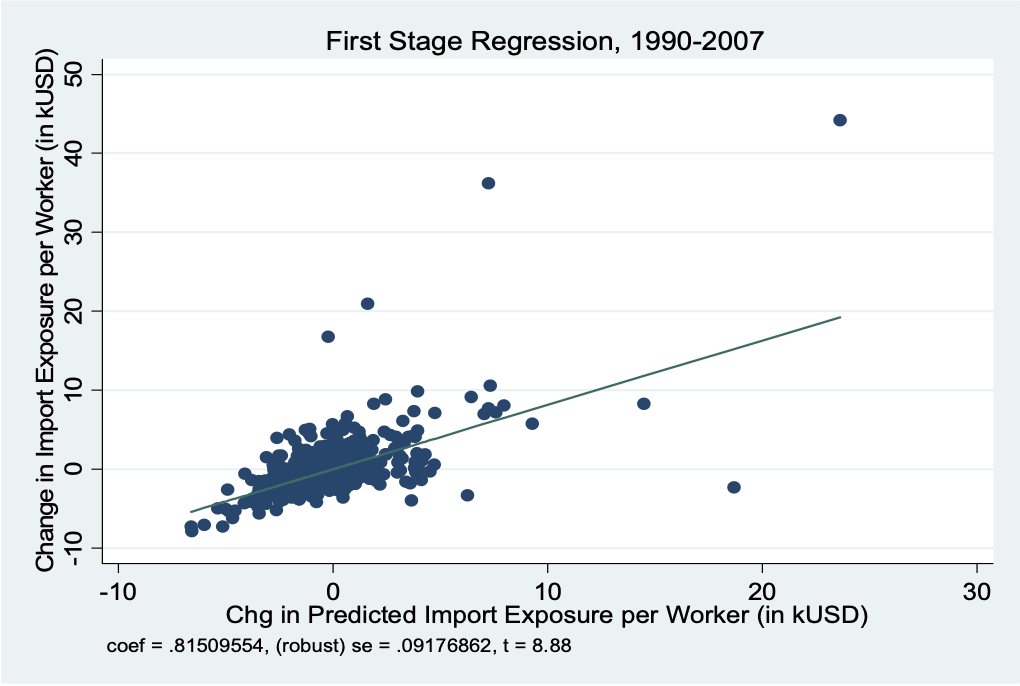
\includegraphics[scale=0.325]{figures/ADHFIG1.png}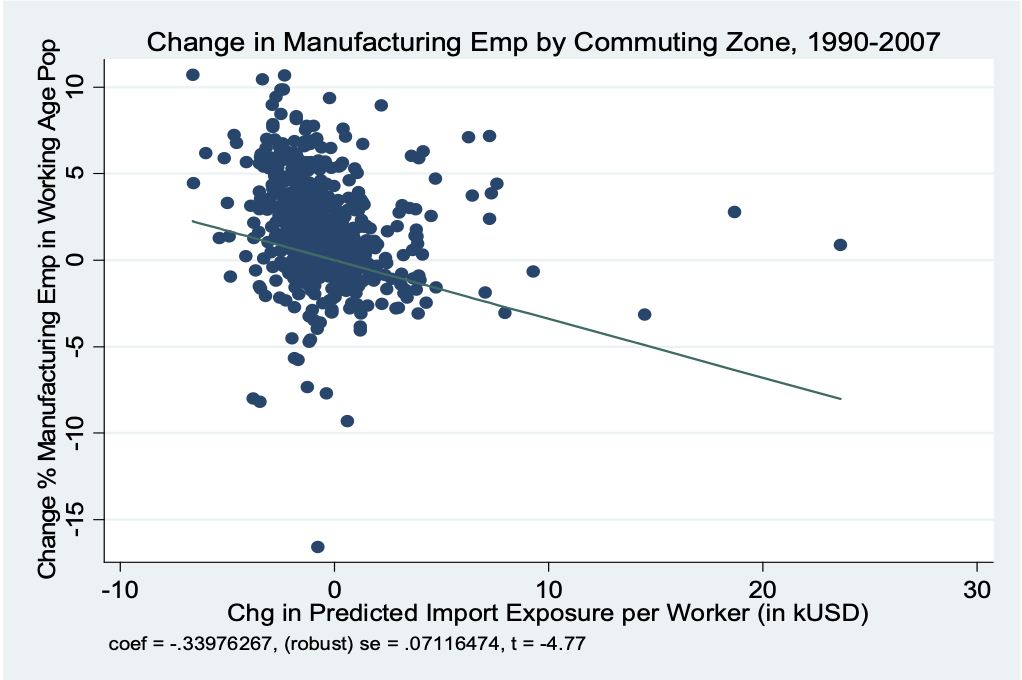
\includegraphics[scale=0.325]{figures/ADHFIG2.png}
\end{frame}


\begin{frame}
\frametitle[alignment=center]{Bartik: Concerns}
Require:
\begin{align*}
%		y_l & = \rho +\beta x_l + \epsilon_l \\
		E(\epsilon_l B_l) = E(\epsilon_l \sum_k z_{l,k}g_k) &= 0  
	\end{align*}
\begin{enumerate}
	\item Pre-shock shares endogenous to lagged shock or the same shock if serially correlated, $E(\epsilon_l  z_{l,k})\neq 0$.
	\begin{itemize}
		\item Random assignment conditional on controls can be difficult to justify: regions that differ in $z$ probably differ on other (unobserved) dimensions too!
	\end{itemize}
	\item National industry shocks correlated with local shocks,
, $E(\epsilon_l  g_k)\neq 0$. 
	\begin{itemize}
		\item In classic Bartik example, worry that $g_k$ is correlated with (unobserved) labor supply shocks.
	\end{itemize}
\end{enumerate}
How to handle identification arguments?
\end{frame}


%%%%%%%%%%%%%%%%%%%%%%%%%%%%%%%%%%%%%%%%%%%%%%%%%%
\section{Goldsmith-Pinkham, Sorkin, and Swift, AER 2020}
%%%%%%%%%%%%%%%%%%%%%%%%%%%%%%%%%%%%%%%%%%%%%%%%%%

\begin{frame}
\frametitle[alignment=center]{Special Case: 2 Industries}
\begin{itemize}
	\item Bartik instrument is proportional to industry share:
	\begin{align*}
		B_l = z_{1l}g_1+z_{2l}g_2 = g_2 + (g_1-g_2)z_{1l}
	\end{align*}
	\item First stage:
	\begin{align*}
		x_l = \gamma_0 + \gamma B_l + \eta_l = \gamma_0 + \gamma g_2 + \gamma (g_1-g_2)z_{1l} + \eta_l 
	\end{align*}
	\item $B_l$ is equivalent to using $z_{1l}$ (or $z_{2l}$) as instrument.
	\item Intution:
	\begin{itemize}
		\item $z_{1l}$ measures exposure, $g_1-g_2$ the magnitude of the treatment.
		\item Many cross-sectional regressions take the view $g_2=0$: heterogeneous exposure to single aggregate shock.
		\item What endogeneity problem does the Bartik instrument (or industry shares) solve? What does it not solve?
	\end{itemize}
\end{itemize}
\end{frame}


\begin{frame}
\frametitle[alignment=center]{General Case (1)}
Notation:
\begin{itemize}
	\item $Z_{lt}=(z_{l1t},...,z_{lkt})$ is a $1\times K$ vector of industry  shares.
	\item $Z_t = (Z_{1t}',...,Z_{Lt}')'$ is a $L\times K$ matrix of industry shares.
	\item $G_{t}=(g_{1t},...,g_{kt})'$ is a $K\times 1$ vector of industry growth rates.
	\item $B_t = Z_0 G_t$ is a $L\times 1$ vector of Bartik instruments.
	\item $X_t=(x_{1t},...,x_{Lt})'$ is a $L\times 1$ vector of endogenous variables.
	\item $Y_t=(y_{1t},...,y_{Lt})'$ is a $L\times 1$ vector of outcomes.
	\item Assume $X_t,Y_t$ previously residualized with respect to any covariates.
\end{itemize}
\end{frame}

\begin{frame}
\frametitle[alignment=center]{General Case (2)}
\begin{itemize}
%	\item 
%	\begin{align*}
%		Z=\begin{pmatrix}
%			Z_0 & 0 & \hdots & 0 \\
%			0 & Z_0 & \hdots & 0 \\
%			\vdots & 0 & \ddots & \vdots \\
%			0 & \hdots & 0 & Z_0 \\
%		\end{pmatrix}
%	\end{align*}
%	\item $G=(G_{1}',...,G_{T})'$ is a $KT\times 1$ vector of industry growth rates.
	\item $B$ is a $LT\times 1$ vector of Bartik instruments.
	\begin{align*}
		B=ZG = \begin{pmatrix}
			Z_0G_1 \\
			Z_0G_2 \\
			\vdots  \\
			Z_0 G_T \\
		\end{pmatrix} =
		\underbrace{\begin{pmatrix}
			Z_0 & 0 & \hdots & 0 \\
			0 & Z_0 & \hdots & 0 \\
			\vdots & 0 & \ddots & \vdots \\
			0 & \hdots & 0 & Z_0 \\
		\end{pmatrix}}_{=Z} \underbrace{\begin{pmatrix}
			G_1 \\
			G_2 \\
			\vdots  \\
			 G_T \\
		\end{pmatrix}}_{=G}
	\end{align*}
	\item $Z$ is a $LT\times KT$ matrix of industry shares
	\item $G$ is a $KT\times 1$ vector of industry growth rates.
	\item $X=(X_{1}',...,X_{T}')'$ is a $LT\times 1$ vector of endogenous variables.
	\item $Y=(Y_{1}',...,Y_{T}')'$ is a $LT\times 1$ vector of outcomes.
	\item The Bartik and GMM estimators are
	\begin{align*}
		\hat{\beta}_{Bartik} = \frac{B'Y}{B'X},\qquad\qquad \hat{\beta}_{GMM}=\frac{X'Z W Z'Y}{X'Z W Z'X}
	\end{align*}
\end{itemize}
\end{frame}

\begin{frame}
\frametitle[alignment=center]{Equivalence of GMM and Bartik}
\begin{itemize}
	\item Proposition: When $W = GG'$ then $\hat{\beta}_{Bartik} = \hat{\beta}_{GMM}$
	\item Proof:
	\begin{align*}
		\hat{\beta}_{GMM} &= (X'Z GG' Z'X)^{-1}(X'Z GG' Z'Y) \\
		&=(X'BB'X)^{-1}(X'BB'Y) \\
		&=(B'X)^{-1}(X'B)^{-1}(X'B)(B'Y)\\
		&=\hat{\beta}_{Bartik}
	\end{align*}
	\item Bartik IV is numerically equivalent to IV regression with $K$ instruments corresponding to the industry shares in $Z$ weighted with industry $GG'$.
	\item More notation extends to case with controls.
\end{itemize}
\end{frame}


\begin{frame}
\frametitle[alignment=center]{Identifying assumptions}
\begin{itemize}
	\item TSLS estimator:
	\begin{align*}
		\hat{\beta} - \beta_0 = \frac{\sum_{t=1}^{T}\sum_{k=1}^K g_{kt} \sum_{l=1}^{L}z_{lk0} \epsilon_{lt}}{\sum_{t=1}^{T}\sum_{k=1}^K g_{kt} \sum_{l=1}^{L}z_{lk0} x_{lt}}
	\end{align*}
	\item Identifying assumption (conditional on observables):
	\begin{align*}
		E\left[\frac{1}{L}\sum_{l=1}^{L}\epsilon_{lt}z_{zlk0}\right] =0,\qquad \forall k, t \\
	\end{align*}
	What are the asymptotics?
	\item $KT$ moment conditions in GMM.
	\item In words: the differential effect of higher exposure of one industry (compared to another) only affects the change in the outcome ($y_{lt}$) through the endogenous variable of interest, and not through any potential confounding channel.
\end{itemize}
\end{frame}


\begin{frame}
\frametitle[alignment=center]{Rotemberg Weights}
\begin{itemize}
	\item In principle, must make exogeneity claim for every industry $k=1,...,k$. Very difficult to do in practice.
	\item GPSS: focus on select industries that are most influential in determining $\hat{\beta}_{Bartik}$.
	\begin{align*}
		\hat{\beta}_{Bartik} = \sum_k \hat{\alpha}_k \hat{\beta}_k
	\end{align*}
	where
	\begin{align*}
		\hat{\beta}_k = (Z_k'X)^{-1}(Z_k'Y),\qquad\qquad \hat{\alpha}_k = \frac{G_k' Z_k'X}{\sum_k G_k' Z_k'X} = \frac{G_k' Z_k'X}{B'X}
	\end{align*}
	\item $\hat{\beta}_k$ is the just-identified IV estimate from using only the industry shares of industry $k$, $Z_k$.
	\item $\hat{\alpha}_k$ are the \emph{Rotemberg Weights}, which sum to 1 (can be negative).
	\begin{itemize}
		\item Contribution of industry $k$ to Bartik first stage covariance. (Not the same as F-stat.)
		\item Measure the sensitivity to bias in instrument $k$.
	\end{itemize}
\end{itemize}
\end{frame}


%%%%%%%%%%%%%%%%%%%%%%%%%%%%%%%%%%%%%%%%%%%%%%%%%%
\section{Borusyak, Hull, and Jaravel, RESTUD 2022}
%%%%%%%%%%%%%%%%%%%%%%%%%%%%%%%%%%%%%%%%%%%%%%%%%%

\begin{frame}
\frametitle[alignment=center]{BHJ Identification}
\begin{itemize}
	\item Bartik = TSLS estimator:
	\begin{align*}
		\hat{\beta} - \beta_0 = \frac{\sum_{t=1}^{T}\sum_{k=1}^K g_{kt} \sum_{l=1}^{L}z_{lk0} \epsilon_{lt}}{\sum_{t=1}^{T}\sum_{k=1}^K g_{kt} \sum_{l=1}^{L}z_{lk0} x_{lt}}
	\end{align*}
	\item Moment condition for identification:
	\begin{align*}
		E\left[\frac{1}{L}\sum_{l=1}^{L}b_{lt} \epsilon_{lt}\right] = E\left[\frac{1}{L}\sum_{l=1}^{L}\left(\sum_{t=1}^{T}\sum_{k=1}^K  g_{kt}z_{lk0}\right) \epsilon_{lt}\right] = 0
	\end{align*}
	\begin{itemize}
		\item GPSS: quasi-random shares $E(\frac{1}{L}\sum_{l}z_{lk0}\epsilon_{lt}|g_{kt})=0$
		\item BHJ approach: quasi-random shocks %$E[\sum_{k}()g_{kt}\epsilon_{lt}|z_{lk0}]=0$
	\end{itemize}
%	\item Quasi-random exposure vs quasi-random shocks.
\end{itemize}
\end{frame}


\begin{frame}
\frametitle[alignment=center]{BHJ Moment Condition}
\begin{itemize}
	\item Moment condition in terms of shocks:
	\begin{align*}
		E\left[\frac{1}{L}B'\epsilon \right] &=  E\left[\frac{1}{L}\sum_{l=1}^{L}\left(\sum_{t=1}^{T}\sum_{k=1}^K  g_{kt}z_{lkt}\right) \epsilon_{lt}\right] \\
		&=E\left[\sum_{k=1}^K \sum_{t=1}^{T}  \underbrace{\left(\frac{1}{L}\sum_{l=1}^{L}z_{lkt}\right)}_{z_{kt}}   g_{kt}   \underbrace{\left(\frac{\frac{1}{L}\sum_{l=1}^{L}z_{lkt}\epsilon_{lt}}{\frac{1}{L}\sum_{l=1}^{L}z_{lkt}}\right)}_{\bar{\epsilon}_{kt}}  \right] \\
		&=E\left[\sum_{k=1}^K \sum_{t=1}^{T} z_{kt}    g_{kt} \bar{\epsilon}_{kt} \right] = E\left[(\check{Z}  G)' \bar{\epsilon} \right] \\
	\end{align*}
	where $\check{Z} = diag(z_{10},...,z_{KT})$.
	\item Interpretation:
	\begin{itemize}
		\item $z_{kt}$ is average exposure to industry $k$.
		\item $\bar{\epsilon}_{kt}$ is exposure-weighted average of shocks to wage growth.
	\end{itemize}
\end{itemize}
\end{frame}


\begin{frame}
\frametitle[alignment=center]{BHJ Proposition 1}
\begin{itemize}
	\item Claim: Bartik IV is equivalent to TSLS with $KT$ excluded instruments $g_{kt}$ and weights $z_{kt}$ in the second-stage regression:
	\begin{align*}
		\bar{y}_{kt} = \alpha + \beta \bar{x}_{kt} + \bar{\epsilon}_{kt}\\
	\end{align*}
	where $\bar{v}_{kt} = \frac{\frac{1}{L}\sum_{l=1}^{L}z_{lkt}v_{lt}}{\frac{1}{L}\sum_{l=1}^{L}z_{lkt}}$.
	\item Proof:
	\begin{align*}
		\hat{\beta}_{Bartik} &= (B'X)^{-1}(B'Y) \\
		&=\left(\sum_{k=1}^K \sum_{t=1}^{T} z_{kt}    g_{kt} \bar{x}_{kt}\right)^{-1}\left(\sum_{k=1}^K \sum_{t=1}^{T} z_{kt}    g_{kt} \bar{y}_{kt}\right) \\
		&= (\check{Z}G'\bar{X})^{-1}(\check{Z}G'\bar{Y}) \\
	\end{align*}
\end{itemize}
\end{frame}




\begin{frame}
\frametitle[alignment=center]{Which case?}
\begin{enumerate}
	\item Exogenous shares: $E\left[\frac{1}{L}\sum_{l=1}^{L}z_{zlk0}\epsilon_{lt}\right] =0$
	\begin{itemize}
		\item Ex ante exposure in location $l$ uncorrelated with unobserved shocks to outcome.
	\end{itemize}
	\item Exogenous shocks (shifters): $E\left[\frac{1}{KT}\sum_{k=1}^K \sum_{t=1}^{T} z_{kt}    g_{kt} \bar{\epsilon}_{kt}\right] =0$
	\begin{itemize}
		\item Shocks to industry $k$ uncorrelated with unobserved industry shocks when weighted by industry size.
	\end{itemize}
\end{enumerate}
\begin{itemize}
	\item What are asymptotics?
	\item Which is more plausible? When?
\end{itemize}
\end{frame}

%%%%%%%%%%%%%%%%%%%%%%%%%%%%%%%%%%%%%%%%%%%%%%%%%%
\section{Borusyak, Hull, WP 2021}
%%%%%%%%%%%%%%%%%%%%%%%%%%%%%%%%%%%%%%%%%%%%%%%%%%

\begin{frame}
\frametitle[alignment=center]{Borusyak, Hull, WP 2021: Non-Random Exposure}
\begin{align*}
		y_i &= \alpha + \beta x_i + \epsilon_i \\
		z_i &= f_i(g,w)
	\end{align*}
\begin{itemize}
	\item Even if shocks are exogenous, $g \perp \epsilon | w$, due to non-random exposure.
\begin{align*}
	E\left[\frac{1}{N}\sum_i z_i \epsilon_i \right] = E\left[\frac{1}{N}\sum_i \mu_i \epsilon_i \right]
\end{align*}
where $\mu_i = E[f_i(g,w)]$.
\item Intuition: some areas systematically get higher / lower treatment due to non-random assignment (exposure).
\item Solution: simulate draws of shocks, compute $\mu_i$, and recenter instrument to $z_i-\mu_i$.
\item A problem for Bartik (inner product) instruments?
\end{itemize}
\end{frame}


\begin{frame}
\frametitle[alignment=center]{Borusyak, Hull, WP 2021: Non-Random Exposure}
\centering
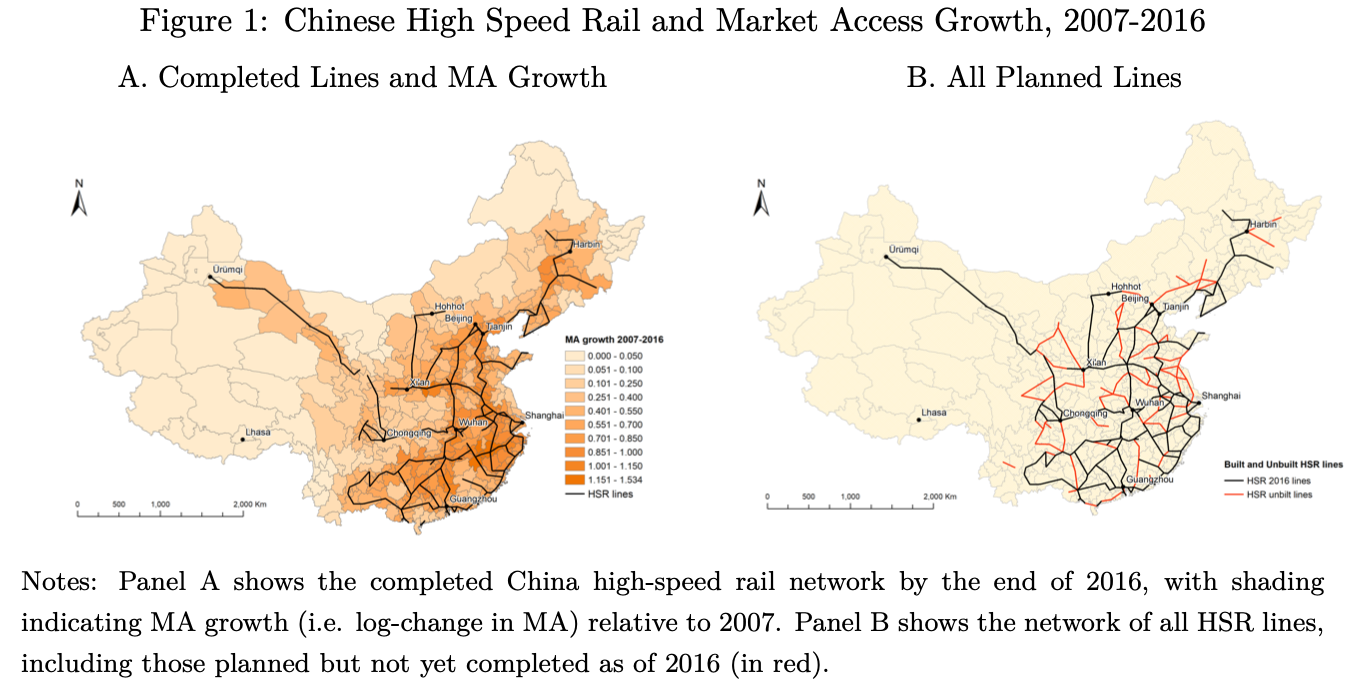
\includegraphics[scale=0.5]{figures/BHFIG1.png}
\end{frame}

\begin{frame}
\frametitle[alignment=center]{Borusyak, Hull, WP 2021: Non-Random Exposure}
\centering
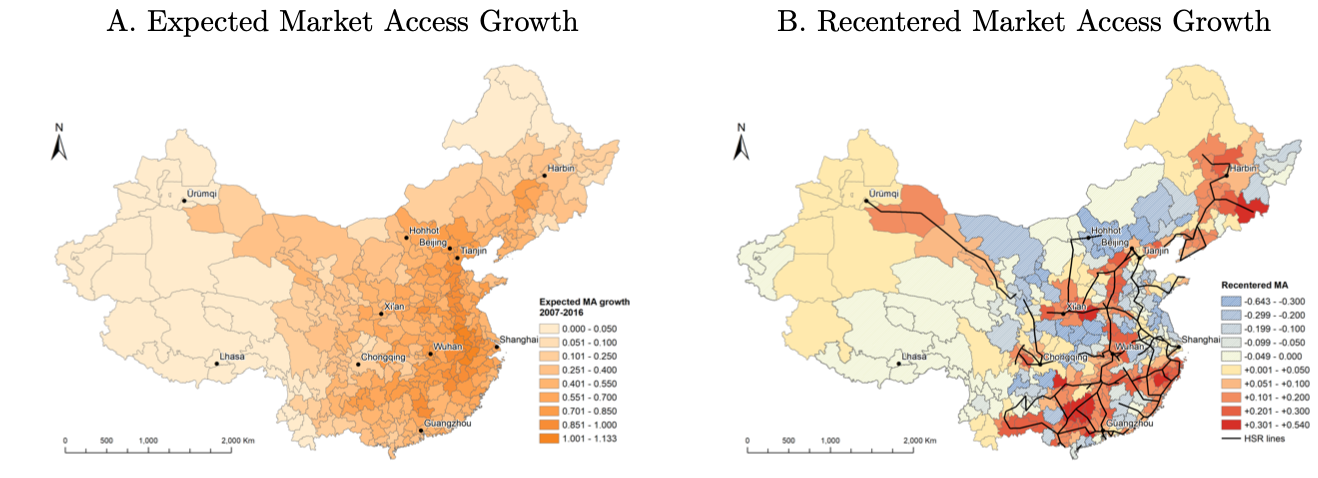
\includegraphics[scale=0.5]{figures/BHFIG2.png}
\end{frame}


%%%%%%%%%%%%%%%%%%%%%%%%%%%%%%%%%%%%%%%%%%%%%%%%%%
\section{More Best Practice}
%%%%%%%%%%%%%%%%%%%%%%%%%%%%%%%%%%%%%%%%%%%%%%%%%%

\begin{frame}
\frametitle[alignment=center]{General Specification Tests}
\begin{enumerate}
	\item Estimated coefficients sensitive to inclusion of covariates?
	\item Pre-trends?
	\item Placebo tests?
	\item Overidentification tests.
	\item Subsample analysis: drop influential observations.
\end{enumerate}
\end{frame}

\begin{frame}
\frametitle[alignment=center]{Leave-one-out}
\begin{itemize}
	\item Typically construct leave-one-out Bartik instrument:
	\begin{align*}
		B_l = \sum_k z_{l,k}g_{-l,k}
	\end{align*}
	\begin{itemize}
		\item $g_{-l,k}$ is national employment growth in industry $k$ excluding area $l$.
	\end{itemize}
	\item Removes finite sample correlation between idiosyncratic industry growth rate $\tilde{g}_{l,k}$ and Bartik instrument $B_l$.
	\item Often unimportant in practice. Why?
\end{itemize}
\end{frame}

\begin{frame}
\frametitle[alignment=center]{Standard Errors}
\begin{itemize}
	\item Ad\~{a}o, Koles\'{a}r, Morales (QJE, 2019): regions with similar exposure are not iid.
	\item Example DGP:
	\begin{align*}
		y_l = \alpha+\beta_0 x_l + \epsilon_l ,\qquad x_l = \sum_k z_{lk}(g_k^1 + g_k^2)
	\end{align*}
	\item Want to know impact of $g^1$ (e.g., China shock):
	\begin{align*}
		y_l = \alpha+\beta_0 \sum_k z_{lk}g_k^1 + (\sum_k z_{lk}g_k^2 + \epsilon_l)
	\end{align*}
	\item Identified if $Cov(\sum_k z_{lk}g_k^1,\sum_k z_{lk}g_k^2 + \epsilon_l) = 0$.
	\item But residuals correlated because of industry structure $\Rightarrow$ need to adjust standard errors. Severity depends on importance of $g_k^2$.
	\item BHJ solve this issue by clustering the industry-level regression.
\end{itemize}
\end{frame}





%%%%%%%%%%%%%%%%%%%%%%%%%%%%%%%%%%%%%%%%%%%%%%%%%%
\section{Nakamura and Steinsson, AER 2014}
%%%%%%%%%%%%%%%%%%%%%%%%%%%%%%%%%%%%%%%%%%%%%%%%%%

\begin{frame}
\frametitle[alignment=center]{Data}
\begin{itemize}
	\item Military procurement data by U.S. State and year.
	\begin{itemize}
		\item  DD-350 military procurement forms
		\item Records purchases $>$ 10k before 1983 and $>25k$ thereafter.
	\end{itemize}	
	\item GDP growth, employment growth, inflation by U.S. State and year.
	\begin{itemize}
		\item How well are these measured?
	\end{itemize}
\end{itemize}
\end{frame}


\begin{frame}
\frametitle[alignment=center]{Specification}
\begin{itemize}
	\item Second stage:
	\begin{align*}
		\frac{Y_{it}-Y_{it-2}}{Y_{it-2}} = \alpha_i + \gamma_t + \beta \frac{G_{it}-G_{it-2}}{G_{it-2}}  + \epsilon_{it}
	\end{align*}
	\item First stage (I):
	\begin{align*}
		\frac{G_{it}-G_{it-2}}{G_{it-2}}  = \delta_i + \theta_t + \sum_k\zeta_k 1(i=k)  \frac{G_{t}-G_{t-2}}{G_{t-2}}  + \eta_{it}
	\end{align*}
	\item First stage (II):
	\begin{align*}
		\frac{G_{it}-G_{it-2}}{G_{it-2}}  = \delta_i + \theta_t + \zeta \left(s_i \frac{G_{t}-G_{t-2}}{G_{t-2}}\right)  + \eta_{it}
	\end{align*}
\end{itemize}
\end{frame}


\begin{frame}
\frametitle[alignment=center]{Identification: Shares or Shocks?}
\emph{Our identifying assumption is that the United States does not embark on military buildups-such as those associated with the Vietnam War and the Soviet invasion of Afghanistan-because states that receive a disproportionate amount of military spending are doing poorly relative to other states.}
\end{frame}

\begin{frame}
\frametitle[alignment=center]{Results}
\centering
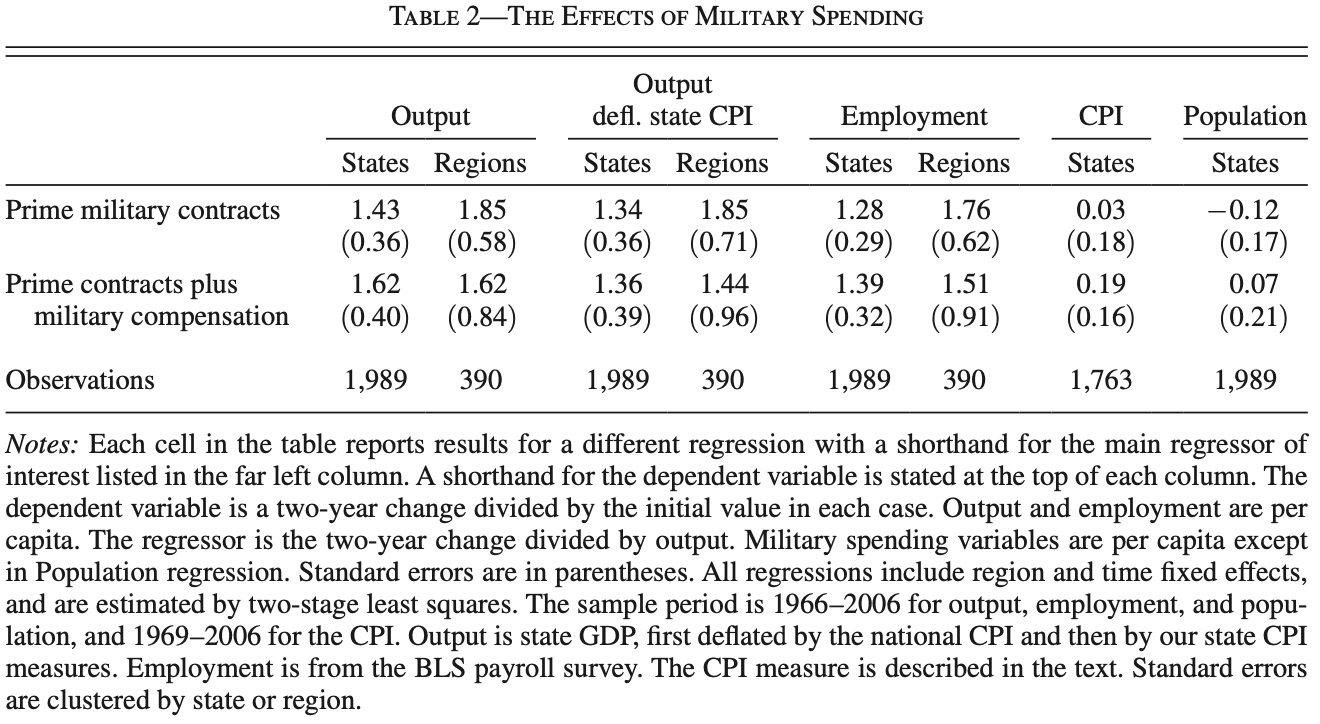
\includegraphics[scale=0.5]{figures/NSTAB2.png}
\end{frame}

\begin{frame}
\frametitle[alignment=center]{Results}
\centering
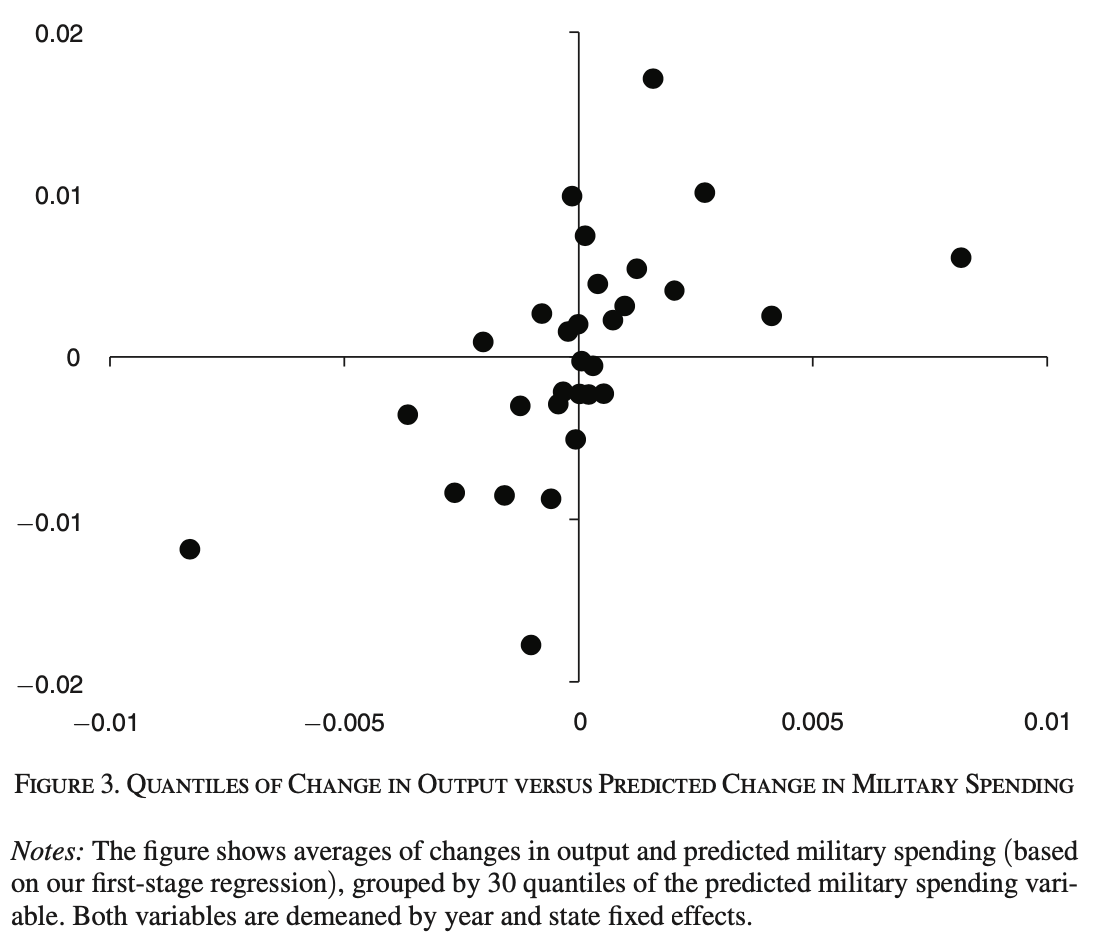
\includegraphics[scale=0.5]{figures/NSFIG3.png}
\end{frame}

\begin{frame}
\frametitle[alignment=center]{Results}
\centering
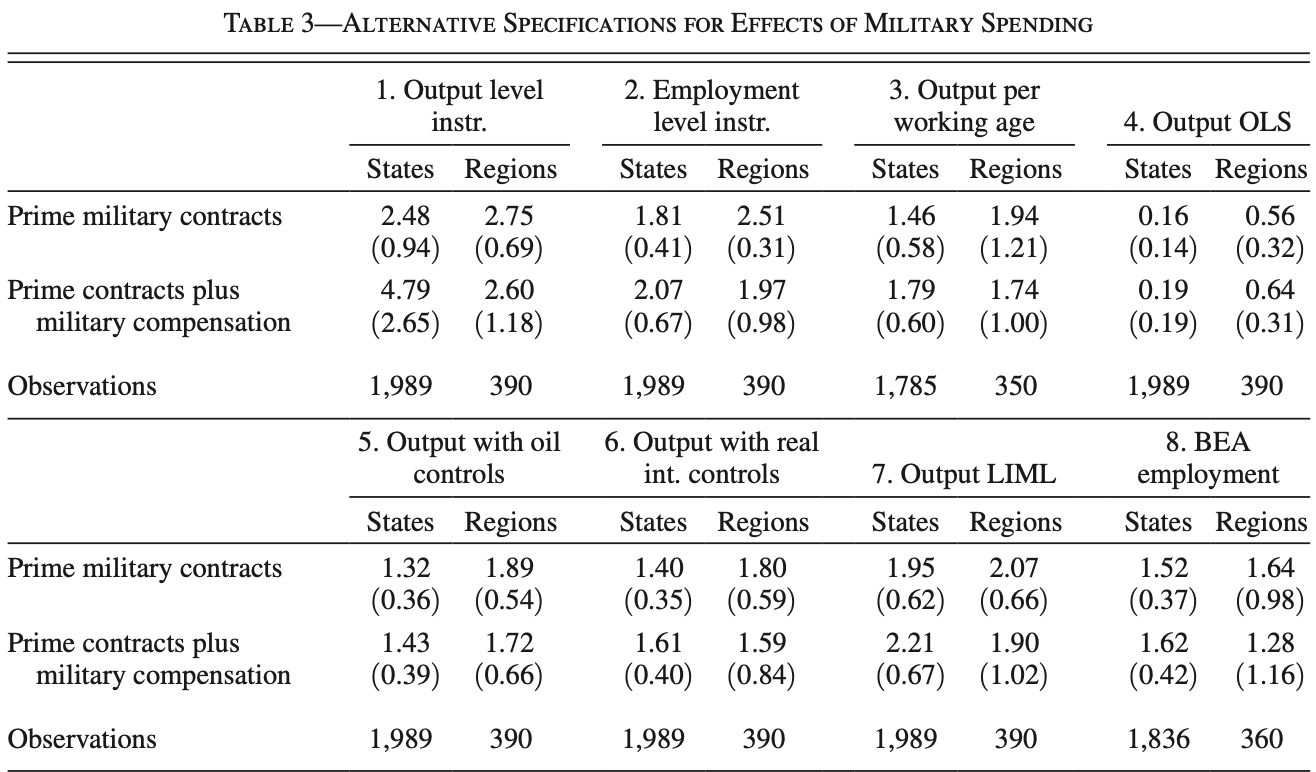
\includegraphics[scale=0.5]{figures/NSTAB3.png}
\end{frame}

\begin{frame}
\frametitle[alignment=center]{What could go wrong?}
\begin{itemize}
	\item What problems do the instrument(s) solve?
	\item What problems remain?
	\item What would you like to see?
\end{itemize}
\end{frame}


%%%%%%%%%%%%%%%%%%%%%%%%%%%%%%%%%%%%%%%%%%%%%%%%%%
\section{Mian, Rao, and Sufi, QJE 2013}
%%%%%%%%%%%%%%%%%%%%%%%%%%%%%%%%%%%%%%%%%%%%%%%%%%


\begin{frame}
\frametitle[alignment=center]{Mian and Sufi}
Establish importance of household debt overhang during Great Recession in a series of papers:\\
\begin{enumerate}
	\item 2009 QJE: Expansion of credit to new subprime borrowers from 2002-2006 led to defaults.
	\item 2011 AER: Credit expansion through home equity borrowing by existing homeowners.
	\item 2013 QJE (with Rao): Consumption and credit crunch 2006-2009.
	\item 2014 Emca: Deleveraging and unemployment, 2006-2009.
	\item 2014 WP: Consumption growth and house prices, 2002-2006.
\end{enumerate}
\end{frame}



\begin{frame}
\frametitle[alignment=center]{Mian, Rao, and Sufi, QJE 2013}
\begin{itemize}
	\item What is the causal effect of changes in net worth on consumption?
	\item Housing net worth shock:
	\begin{align*}
		\frac{\Delta \log p^H_{i,06-09}H_{i,2006}}{NW_{i,2006}}
	\end{align*}
	\item Regression:
	\begin{align*}
		\Delta log C_{i,06-09} = \alpha_t + \beta \frac{\Delta \log p^H_{i,06-09}H_{i,2006}}{NW_{i,2006}} + \gamma X_{it} + \epsilon_{it}
	\end{align*}
	\item Identification assumption?
%	the cross-sectional variation in housing wealth is not spuriously correlated with industry-specific shocks, such as the construction sector.
\end{itemize}
\end{frame}

\begin{frame}
\frametitle[alignment=center]{Data}
\begin{itemize}
	\item County-level total consumer purchases with a credit card or debit card for which MasterCard is the processor by NAICS code. 
	\begin{itemize}
		\item Combine with census retail sales data.
	\end{itemize}
	\item ZIP code-level auto sales data.
	\item ZIP code-level net worth:
	\begin{align*}
		NW_{it} = S_{it} + B_{it} + H_{it} - D_{it}
	\end{align*}
	\begin{itemize}
		\item IRS Statistics of Income (SOI) to proxy for $S_{it}, B_{it}$
		\item Core Logic ZIP code-level house price index to get $H_{it}$.
		\item Equifax Predictive Services to measure $D_{it}$
	\end{itemize}
\end{itemize}
\end{frame}

\begin{frame}
\frametitle[alignment=center]{Large Variation in Net Worth}
\centering
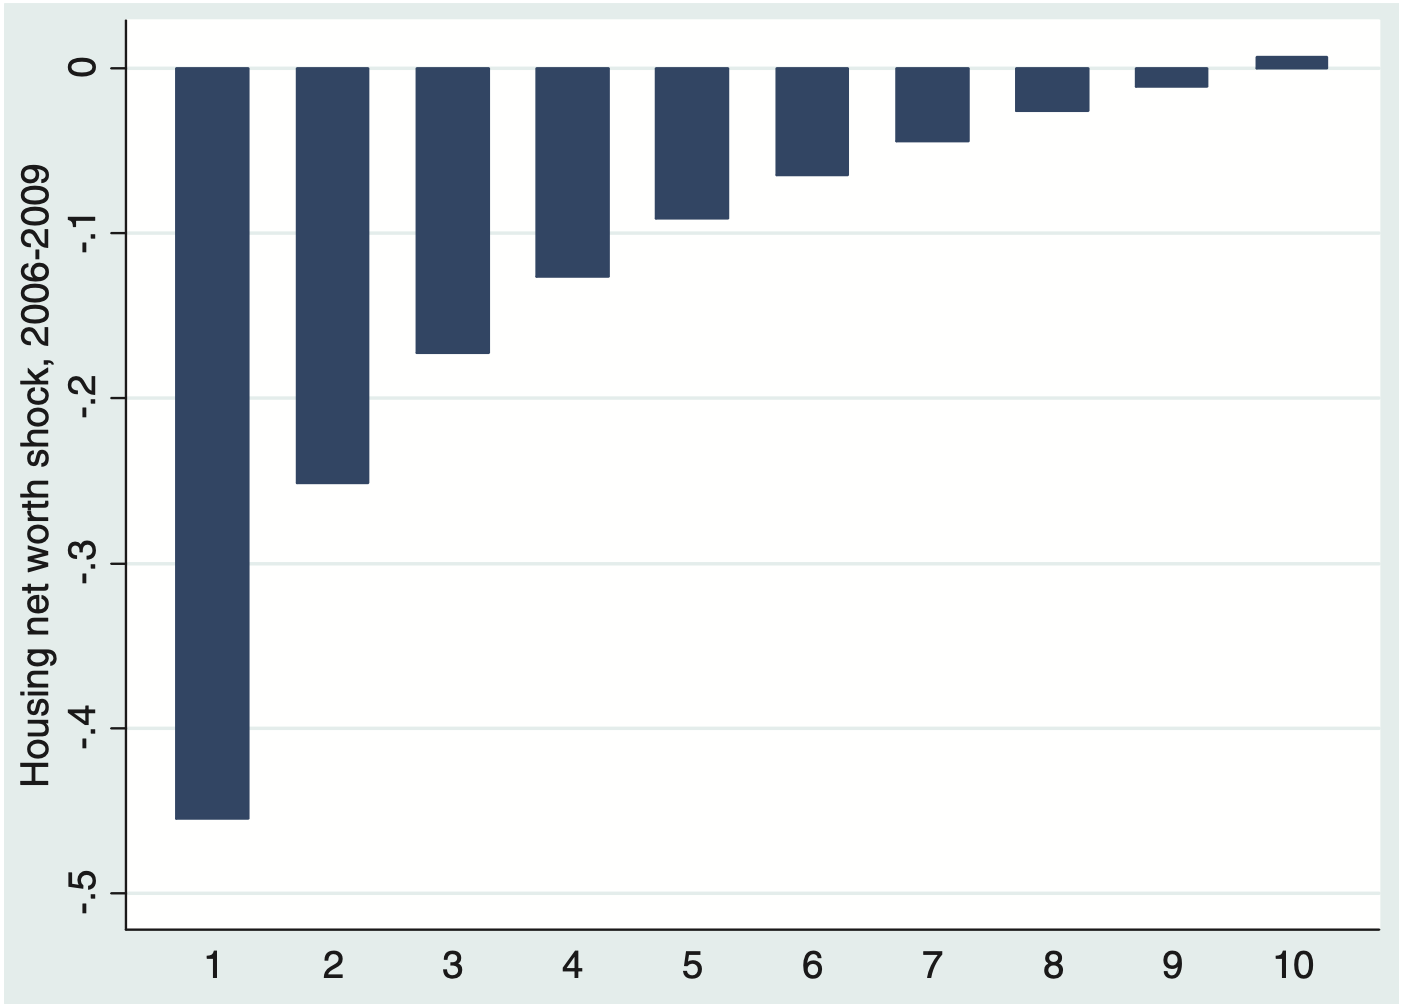
\includegraphics[scale=0.4]{figures/MRSFIG2.png}
\end{frame}

\begin{frame}
\frametitle[alignment=center]{Correlated with Housing Supply Instrument}
\centering
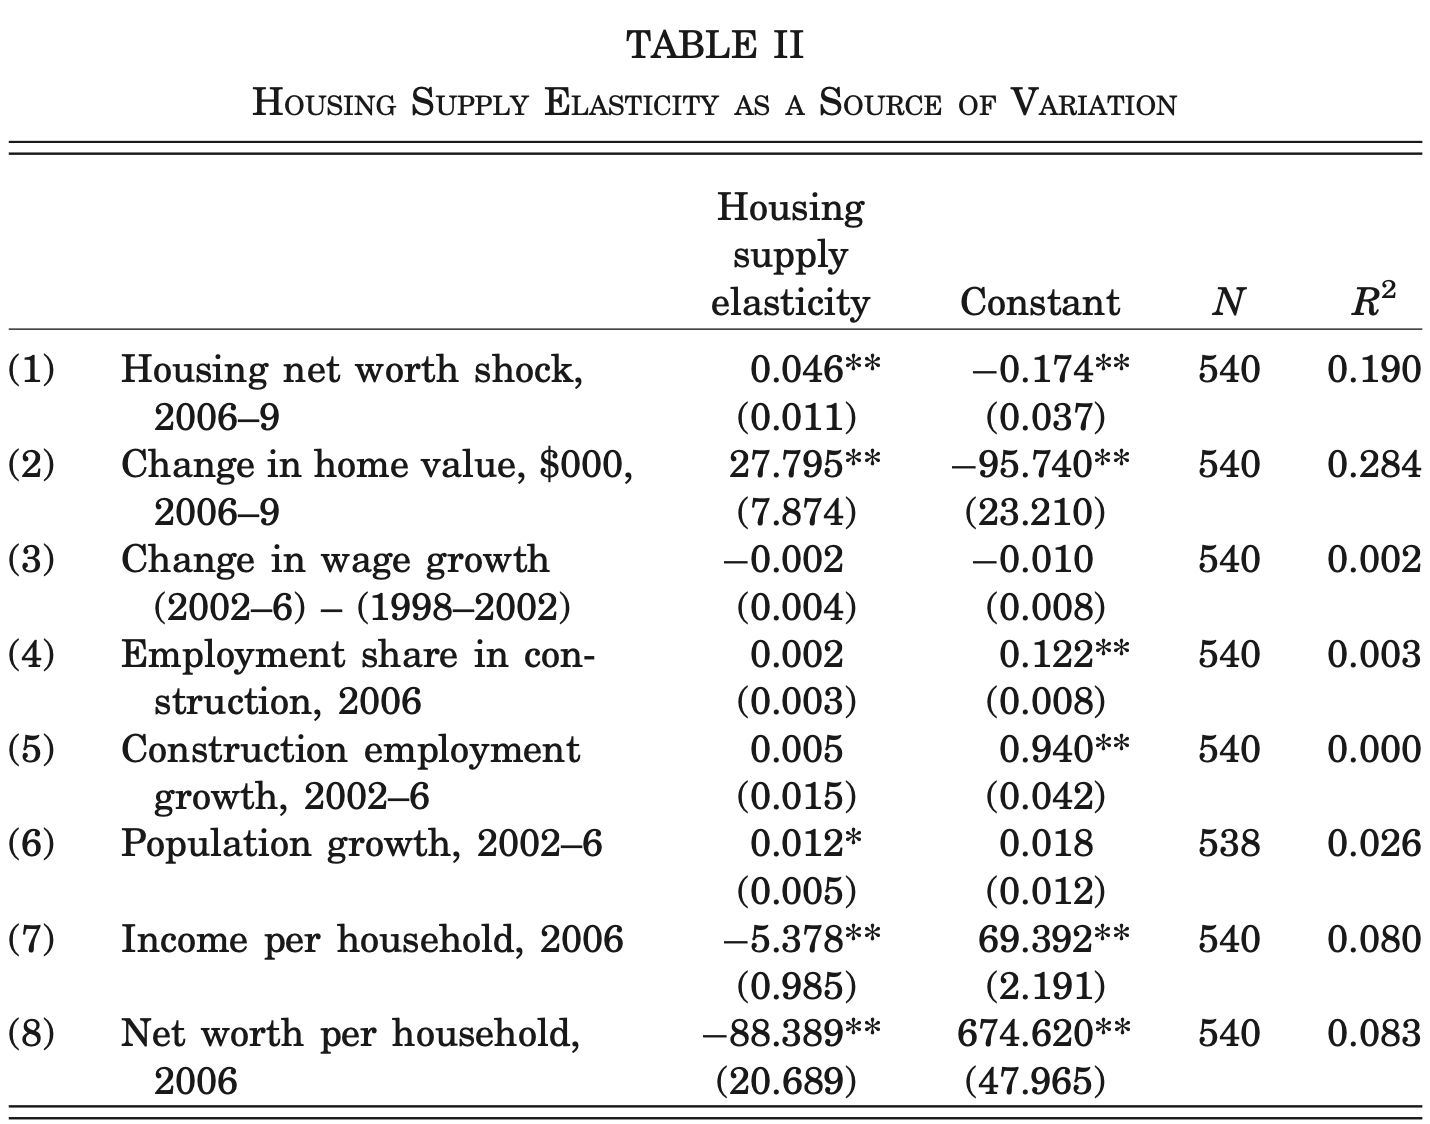
\includegraphics[scale=0.4]{figures/MRSTAB2.png}
\end{frame}

\begin{frame}
\frametitle[alignment=center]{Net Worth Decline Predicts Spending Decline}
\centering
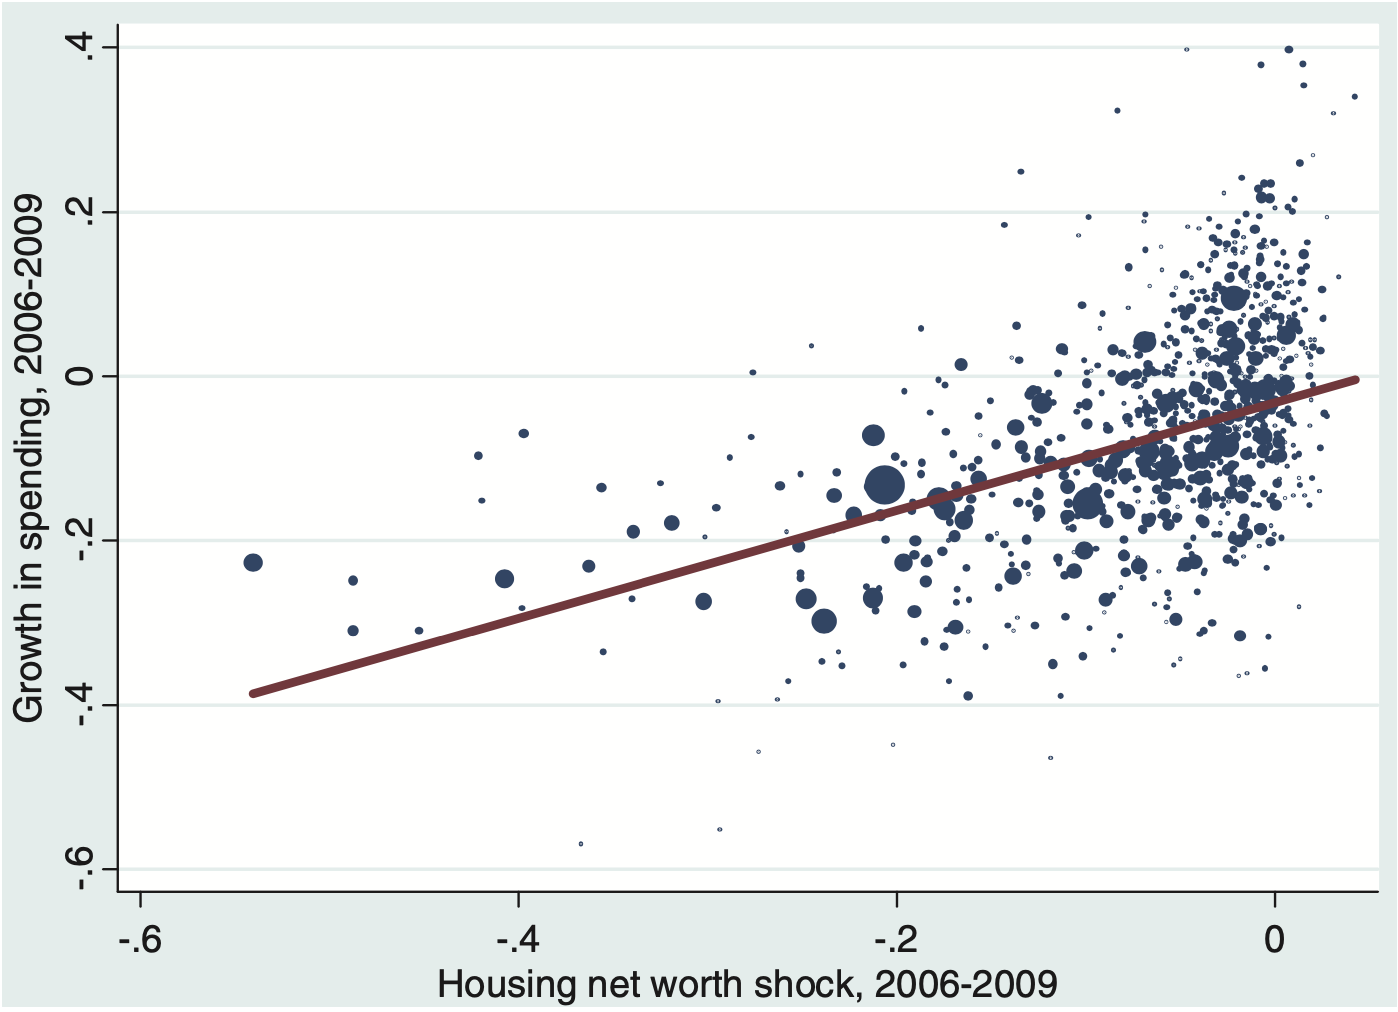
\includegraphics[scale=0.4]{figures/MRSFIG3.png}
\end{frame}

\begin{frame}
\frametitle[alignment=center]{Net Worth Decline Predicts Spending Decline}
\centering
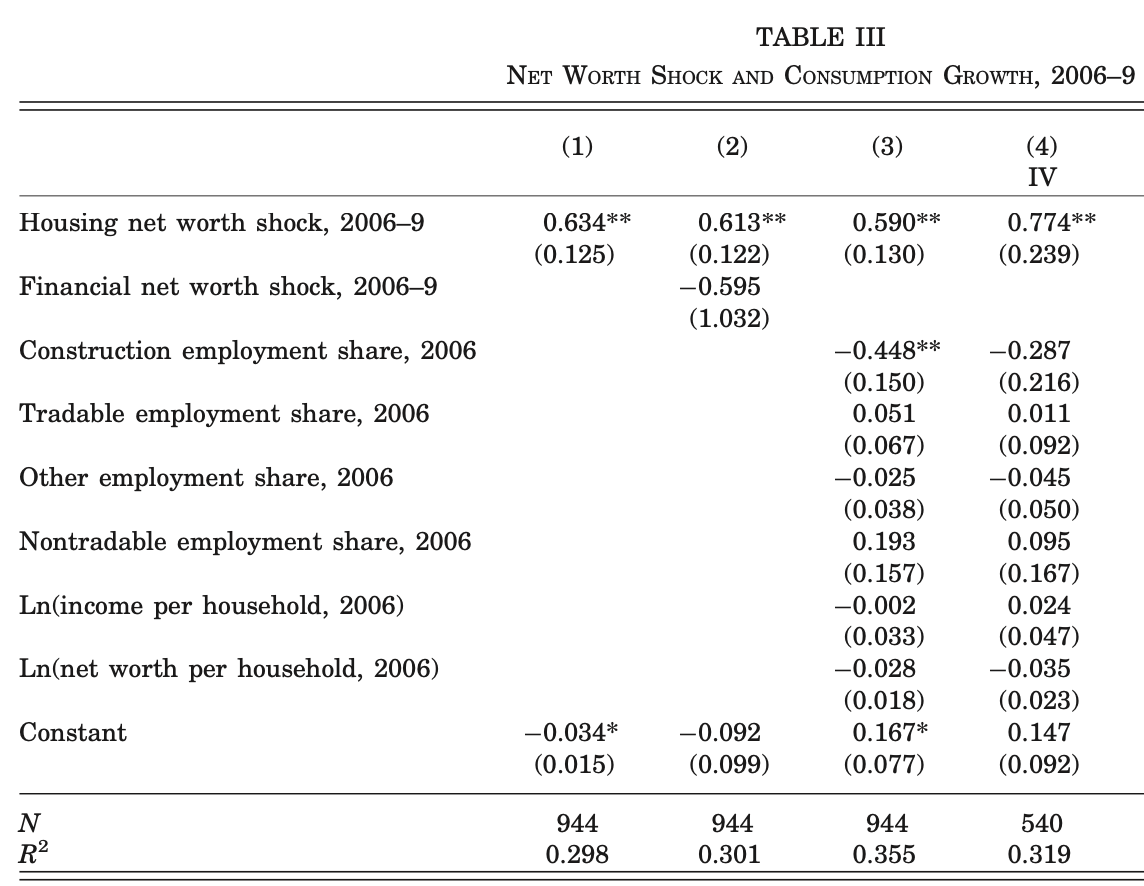
\includegraphics[scale=0.5]{figures/MRSTAB3.png}
\end{frame}

\begin{frame}
\frametitle[alignment=center]{MPC}
\centering
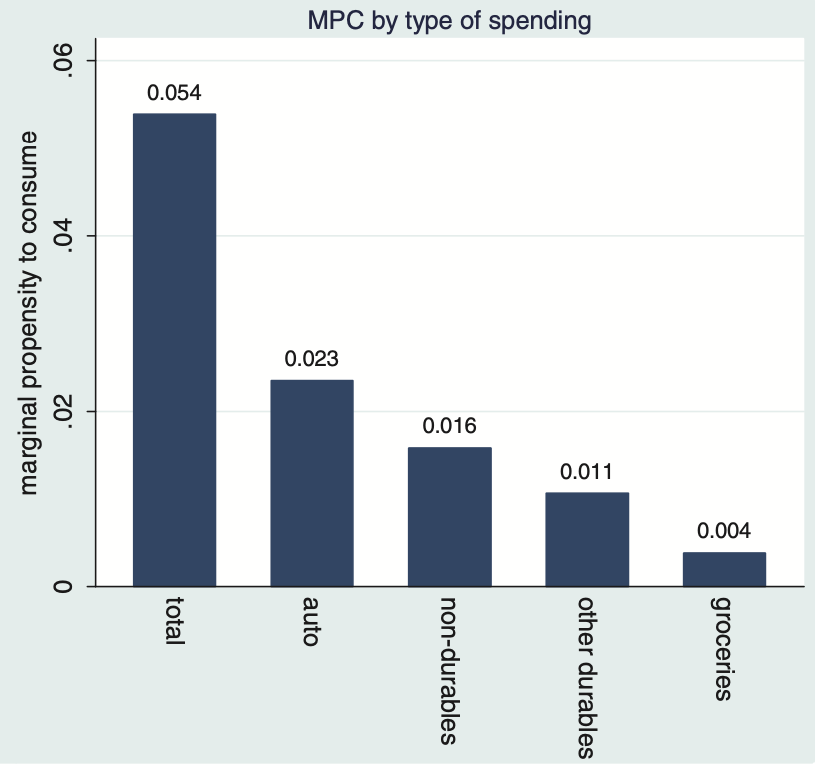
\includegraphics[scale=0.6]{figures/MRSFIG4b.png}
\end{frame}

\begin{frame}
\frametitle[alignment=center]{What could go wrong?}
\begin{itemize}
	\item What problems do the instrument(s) solve?
	\item What problems remain?
	\item What would you like to see?
\end{itemize}
\end{frame}


\begin{frame}
\frametitle[alignment=center]{Heterogeneity in MPC}
\begin{itemize}
	\item Does MPC differ by household wealth, income, and / or leverage?
	\item Specification:
	\begin{align*}
		\Delta C_{i,06-09} &= \alpha_t + \beta_1 \Delta  p^H_{i,06-09}H_{i,2006} + \beta_2 Z_{i,t-1} \\
		& \;+ \beta_3  \Delta  p^H_{i,06-09}H_{i,2006} Z_{t-1}  + \gamma X_{it} + \epsilon_{it} \\
	\end{align*}
	where $Z_{i,t-1} = NW_{i,2006}$, $Z_{i,t-1} = INC_{i,2006}$ or $Z_{i,t-1} = LTV_{2006}$
	\item Identification assumption?
\end{itemize}
\end{frame}


\begin{frame}
\frametitle[alignment=center]{Heterogeneity by Income}
\centering
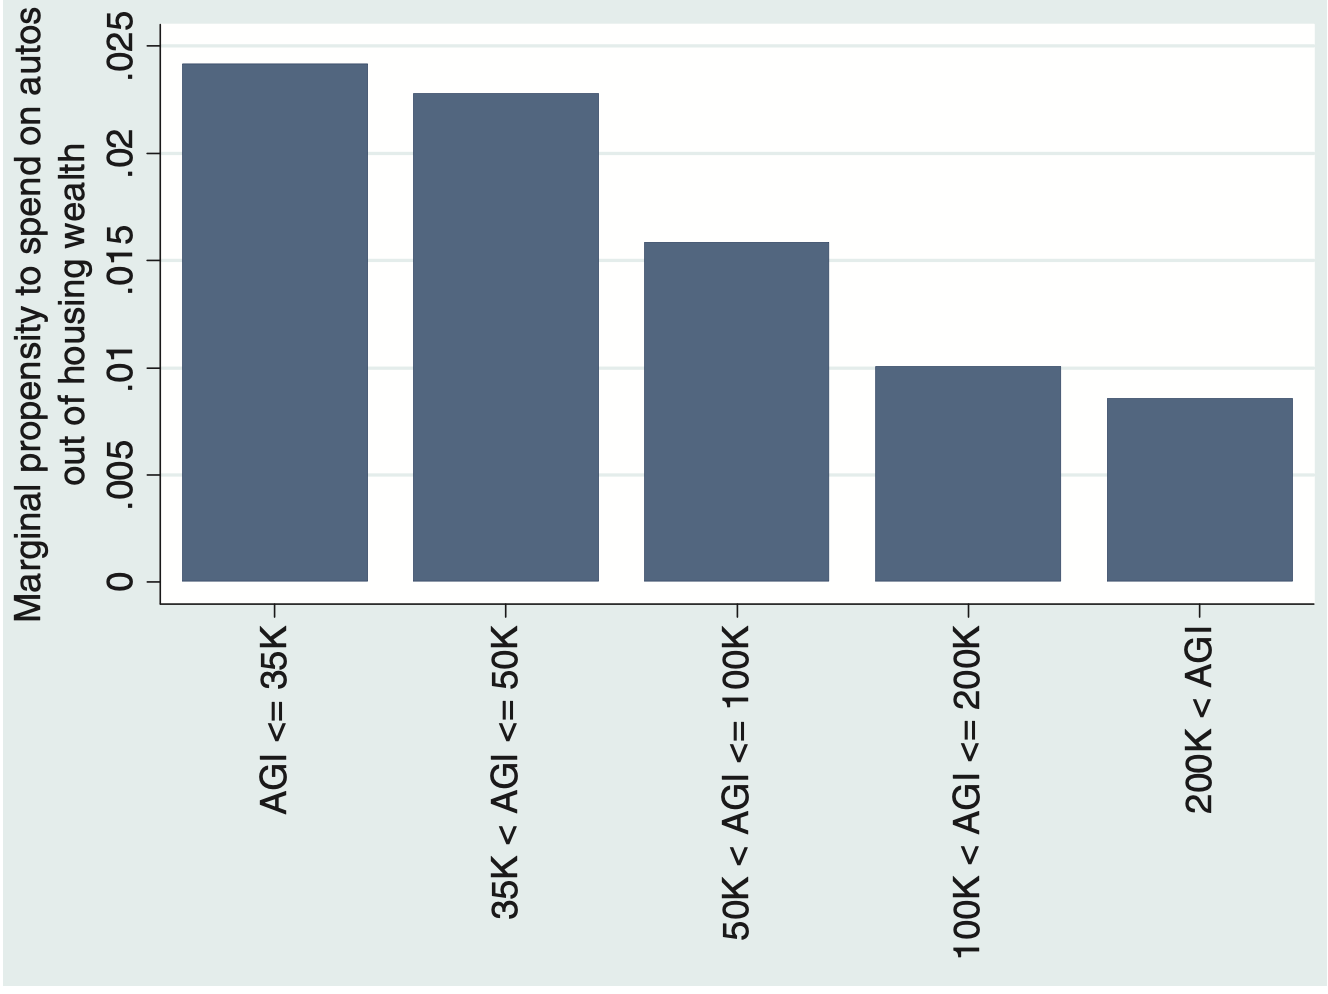
\includegraphics[scale=0.4]{figures/MRSFIG5.png}
\end{frame}

\begin{frame}
\frametitle[alignment=center]{Heterogeneity by Leverage}
\centering
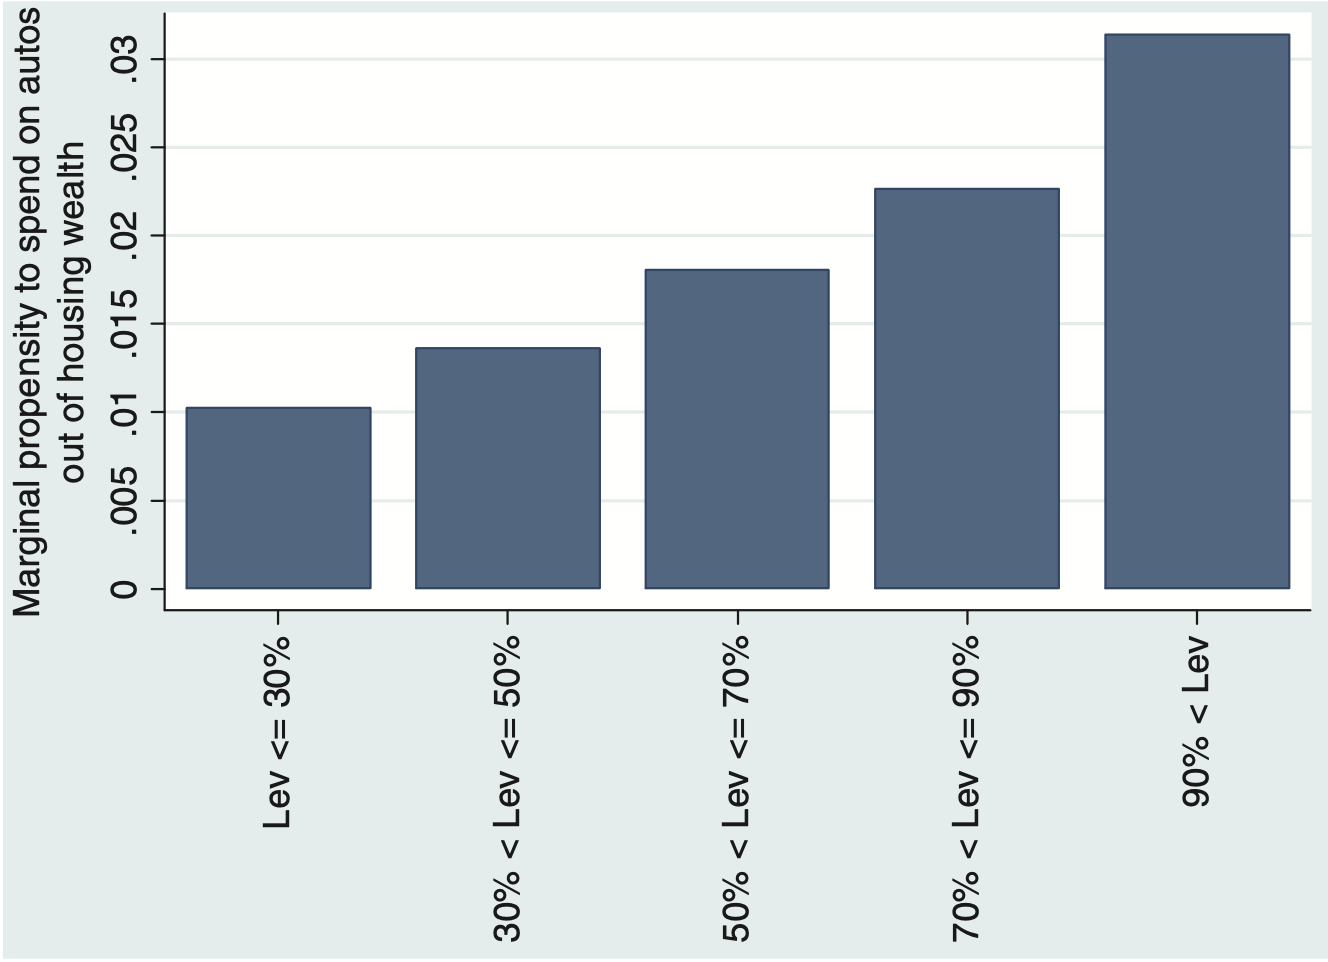
\includegraphics[scale=0.4]{figures/MRSFIG6.png}
\end{frame}

\begin{frame}
\frametitle[alignment=center]{Mechanism}
\centering
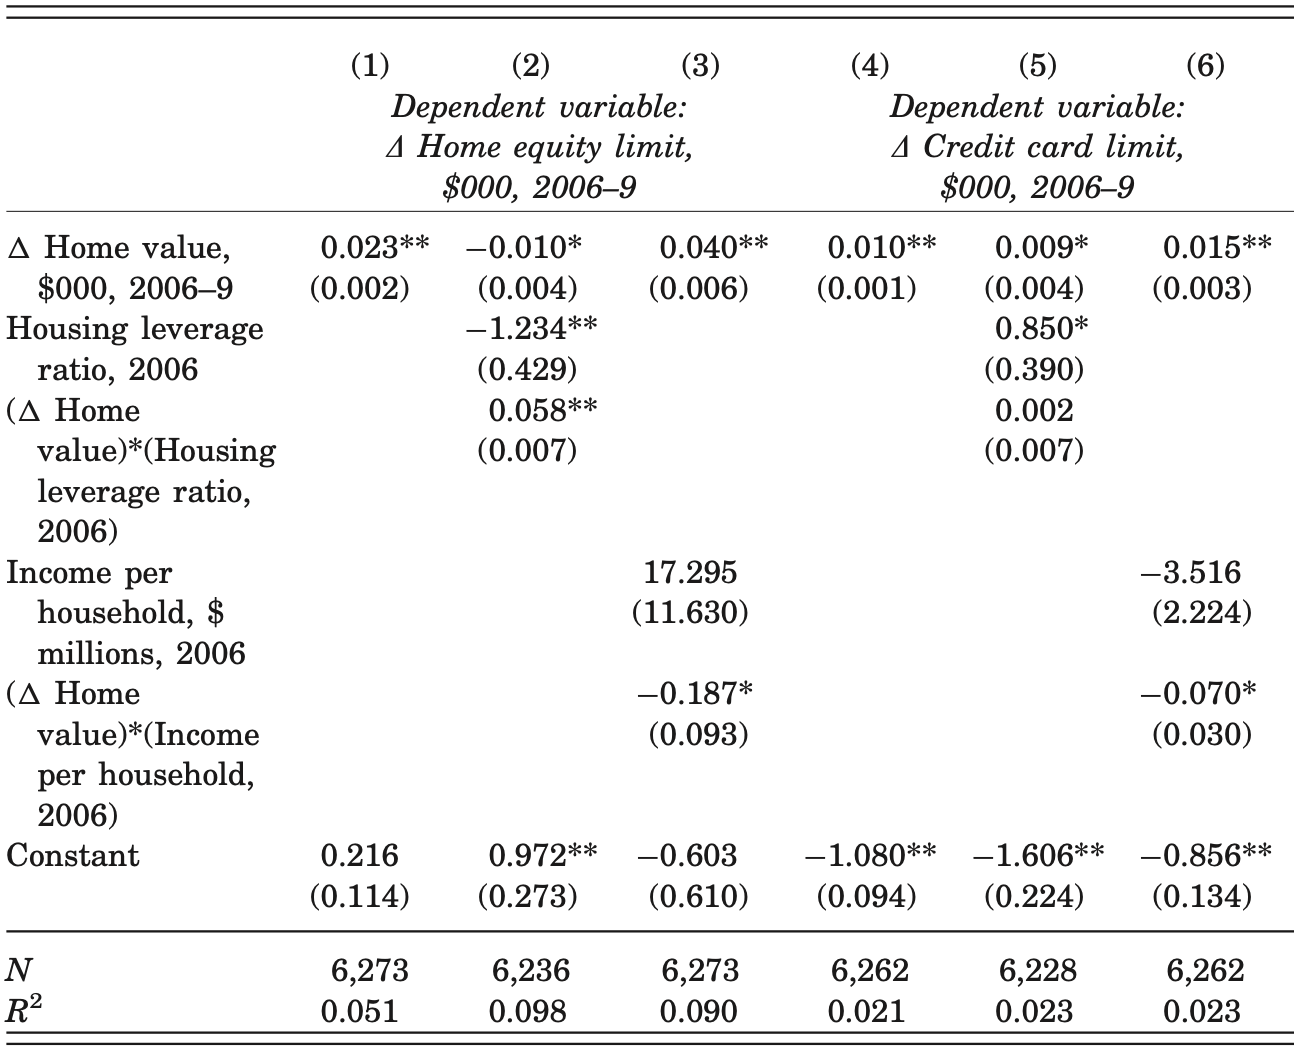
\includegraphics[scale=0.4]{figures/MRSTAB7a.png}
\end{frame}

\begin{frame}
\frametitle[alignment=center]{Convincing?}

\end{frame}




\end{document}